\chapter{Nanopore Signal Analysis}
\label{cha:signal}

\begin{figure}[h]
    \centering
    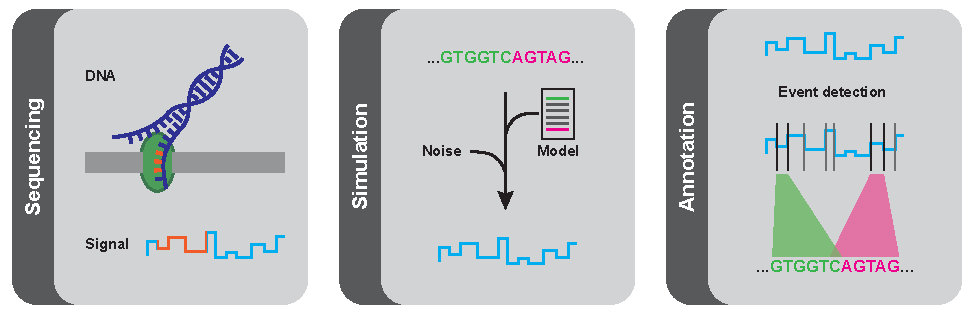
\includegraphics[width=1.0\textwidth]{figures/signal/GA.pdf}
    \label{fig:signal:ga}
\end{figure}

\begin{itemize}
	\item basic framework for development set with pipeline
	\item need to understand signal, contrast to 2nd gen.
	\item tombo, squiggle-kit? available, but not customizable regarding normalization, parameter etc.
	\item need for custom, easy to configure, python for fast prototyping
	\item fast5 format, hdfviewer, BulkVis as basic tools to work with fast5 files
\end{itemize}

\section{Simulation}
\label{sec:signal:simulation}

\begin{itemize}
    \item basic pore model
    \item base mod pore model
    \item trace with constant, time warping and noise
    \item more sophisticated simulation with simulatION, deepSimulator, scrappie, etc.
\end{itemize}


\begin{figure}[h]
	\centering
	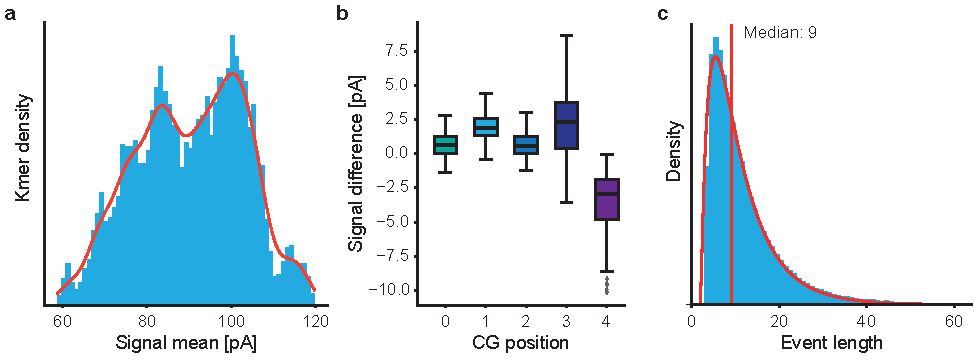
\includegraphics[width=1.0\textwidth]{figures/signal/pm.pdf}
	\captionsetup{format=plain}
	\caption[Pore model and event length]{Pore model and event lengths: \textbf{a}, Density plot and kernel density estimation of expected signal levels per kmer (k=6, n=4096, mean ionic current in pA). \textbf{b}, Expected signal difference of native and 5mC modified DNA for 6mers with single CG (n=256 per position) depending on the CG location. \textbf{c}, Event length (samples per kmer) density plot from signal alignment (approximated by generalized gamma distribution with a=4.3, c=0.6, shit=2, scale=0.7).}
	\label{fig:signal:pm}
\end{figure}

\begin{figure}[h]
	\centering
	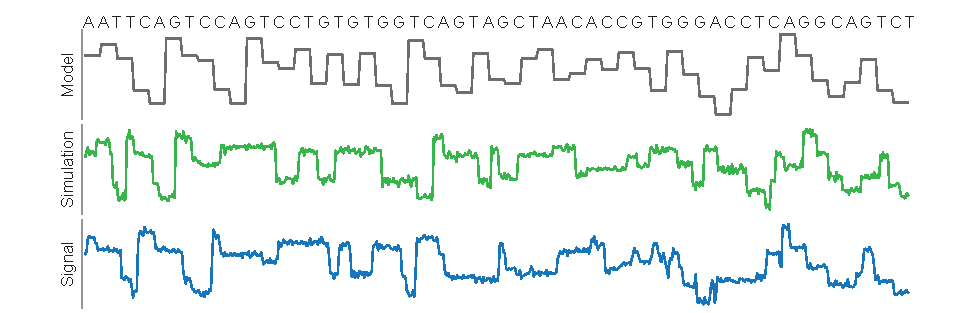
\includegraphics[width=1.0\textwidth]{figures/signal/simulation.pdf}
	\captionsetup{format=plain}
	\caption[Basic signal simulation]{Basic nanopore signal simulation from pore model and event lengths: Mean ionic current levels per kmer for short sequence (top), simulated nanopore signal with noise and random time warping (center) and raw signal fragment extracted from real nanopore read covering the same sequence (bottom).}
	\label{fig:signal:simulation}
\end{figure}




\section{Normalization}
\label{sec:signal:normalization}

\begin{itemize}
	\item mean/std vs median/MAD (cite tombo)
	\item min-max normalization with repeat signals in mind
	\item smoothing with grayscale morphological operations
	\item histogram equalization to deal with bimodal distribution of raw signal
\end{itemize}


\begin{figure}[h]
	\centering
	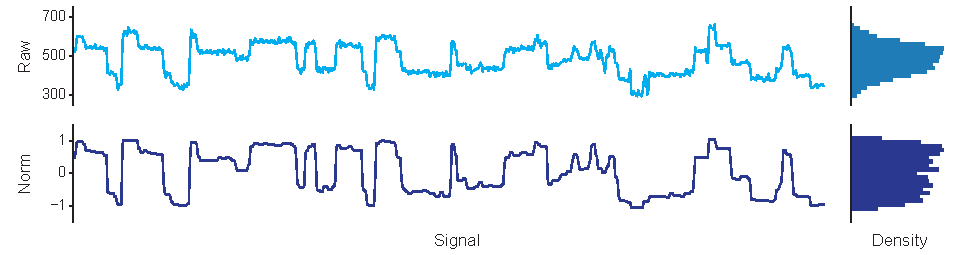
\includegraphics[width=1.0\textwidth]{figures/signal/normalization.pdf}
	\captionsetup{format=plain}
	\caption[Signal normalization and histogram equalization]{Raw signal normalization and histogram equalization.}
	\label{fig:signal:normalization}
\end{figure}


\section{Alignment and Segmentation}
\label{sec:signal:alignment}

\begin{itemize}
	\item raw signal alignment with seqan based scoring and semi-global dp
	\item segmentation with basic image processing tools, edge filter + threshold
	\item event alignment with edlib to be more robust against time-warping
	\item profile HMM for most precise mapping
\end{itemize}

\begin{equation}
s_{i,j} = max \left\lbrace c - \left| x_{i} - y_{j} \right| \atop -c \right.
\end{equation}

\begin{table}[ht]
	\centering
	\caption[Event detection and annotation]{Event summary of raw nanopore signal with reference sequence annotation.}
	\label{tab:signal:events}
	\begin{tabular}{l|r|r|r|l}
		 & mean & event length & seq. offset & kmer \\
		\hline 
		& \multicolumn{3}{c|}{...} &  \\
		\hline
		$ E_{n} $ &  1.332  & 15 & 3205 & AGTCCA \\
		\rowcolor{LightOrange}
		$ E_{n+1} $ &  0.981  & 22 & 3206 & GTCCAG \\
		$ E_{n+2} $ & -1.058  &  6 & 3208 & CCAGTC \\
		$ E_{n+3} $ & -1.662  & 17 & 3209 & CAGTCC \\
		$ E_{n+4} $ &  1.360  &  7 & 3210 & AGTCCT \\
		$ E_{n+5} $ &  0.664  & 33 & 3211 & GTCCTG \\
		$ E_{n+6} $ &  0.107  & 11 & 3212 & TCCTGT \\
		\rowcolor{LightGreen}
		$ E_{n+7} $ &  0.844  &  4 & 3213 & CCTGTG \\
		\rowcolor{LightGreen}
		$ E_{n+8} $ &  1.362  & 38 & 3213 & CCTGTG \\
		\hline
		& \multicolumn{3}{c|}{...} &  \\
	\end{tabular} 
\end{table}


\cite{Schreiber2015}

\begin{figure}[h]
	\centering
	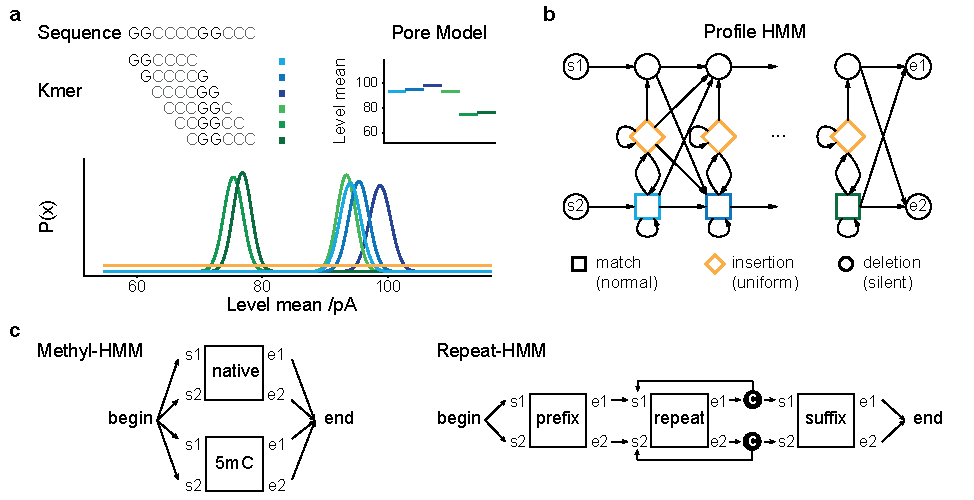
\includegraphics[width=1.0\textwidth]{figures/signal/count_hmm.pdf}
	\captionsetup{format=plain}
	\caption[Nanopore signal processing with STRique]{\textbf{a}, A compound profile HMM of prefix, a single repeat and the suffix sequence assigns either prefix, repeat or suffix label to each signal value. Repeat counts are obtained through dummy states between repeat and suffix. \textbf{b}, Nanopore signal profile HMM with normal distributed match state and uniform distributed insertion state emission probabilities.}
	\label{fig:strique:count_hmm}
\end{figure}



